\chapter{Proposed methods}
\label{ch:methods}

In this section I will describe the methods I am employing in my research with some sections intentionally brief.
This section is heavily supplemented by publications included as appendices to this document.

\section{Deterministic transport}

For deterministic methods appendix \ref{app:therefore} contains, expanded derivations of the higher order space-time-energy discretization scheme, derivation of Fourier analysis of the discretization scheme, derivation of the method of manufactured solution, and description of the implementation in code.
The remainder of this section will be devoted to describing the current state of the investigations into an acceleration scheme for OCI in the thin limit (see section \ref{ssec:method_acc}).

\subsection{Derivation of Higher order Methods in Iterative Schemes}

When the S$_N$ transport equation is descritzed in space using simple corner balance and in time with time dependent multiple balance a 4-equation system is begot:
\begin{subequations}
    \label{eq:tdmb+scb}
    \begin{multline}
    \label{eq:scb-mb-a}
    \frac{\Delta x_j}{2} \frac{1}{v_g} \left( \frac{\psi_{m,g,k+1/2,j,L} - \psi_{m,g,k-1/2,j,L}}{\Delta t} \right) \\
     + \mu_m \left[ \frac{\left( \psi_{m,g,k,j,L} + \psi_{m,g,k,j,R} \right)}{2}  - \psi_{m,g,k,j-1/2} \right] \\
    + \frac{\Delta x_j}{2} \Sigma_{j} \psi_{m,g,k,j,L} 
    = \frac{\Delta x_j}{2} \frac{1}{2} \left( \sum\limits_{g' = 0}^G \Sigma_{s,j, g'\to g}(x) \sum\limits_{n=1}^N w_n \psi_{n,g,k,j,L} + Q_{k,j,L} \right) \;,
    \end{multline}  
    \begin{multline}
    \label{eq:scb-mb-b}
    \frac{\Delta x_j}{2} \frac{1}{v} \left( \frac{\psi_{m,k+1/2,j,R} - \psi_{m,k-1/2,j,R}}{\Delta t} \right) + \\
    \mu_m \left[ \psi_{m,k,j+1/2} - \frac{\left( \psi_{m,k,j,L} + \psi_{m,k,j,R} \right)}{2}   \right] \\
    + \frac{\Delta x_j}{2} \Sigma_{j} \psi_{m,k,j,R} = \frac{\Delta x_j}{2} \frac{1}{2} \left( \sum\limits_{g' = 0}^G \Sigma_{s,j, g'\to g} \sum\limits_{n=1}^N w_n \psi_{n,g',k,j,R} + Q_{k,j,R} \right) \;,
    \end{multline}  
    \begin{multline}
    \label{eq:scb-mb-c}
    \frac{\Delta x_j}{2} \frac{1}{v_g} \left( \frac{\psi_{m,g,k+1/2,j,L} - \psi_{m,g,k,j,L}}{\Delta t/2} \right) \\
    + \mu_m \left[ \frac{\left( \psi_{m,g,k+1/2,j,L} + \psi_{m,g,k+1/2,j,R} \right)}{2}  - \psi_{m,g,k+1/2,j-1/2} \right]\\
    + \frac{\Delta x_j}{2} \Sigma_{j} \psi_{m,g,k+1/2,j,L} = \frac{\Delta x_j}{2} \frac{1}{2} \left( \sum\limits_{g' = 0}^G \Sigma_{s,j, g'\to g} \sum\limits_{n=1}^N w_n \psi_{n,g',k+1/2,j,L} + Q_{k+1/2,j,L} \right) \;,
    \end{multline}    
    \begin{multline}
    \label{eq:scb-mb-d}
    \frac{\Delta x_j}{2} \frac{1}{v_g} \left( \frac{\psi_{m,g,k+1/2,j,R} - \psi_{m,g,k,j,R}}{\Delta t/2} \right) + \\
    \mu_m \left[ \psi_{m,g,k+1/2,j+1/2} - \frac{\left( \psi_{m,g,k+1/2,j,L} + \psi_{m,g,k+1/2,j,R} \right)}{2}   \right]  \\
    + \frac{\Delta x_j}{2} \Sigma_{j} \psi_{m,g,k+1/2,j,R} = \frac{\Delta x_j}{2} \frac{1}{2} \left( \sum\limits_{g' = 0}^G \Sigma_{s,j, g'\to g} \sum\limits_{n=1}^N w_n \psi_{n,g',k+1/2,j,R} + Q_{k+1/2,j,g,R} \right) \;,
    \end{multline} 
\end{subequations}

where $\Delta x$ is the cell width, $j$ is the spatial index, $L$ and $R$ denote the right and left half-cell averaged quantities, $k$ is time averaged quantities, $k+1/2$ is time edge quantities.
These equations contain a spatial---the angular flux at the cell midpoint is a simple average of the two half-cell average quantities---and a time---\textit{upstream} prescription for the cell-edge angular flux---closures.
This defines system defines angular flux on a stencil shown in figure \ref{fig:stencil}.

\begin{figure}[!htb]
    \centering
    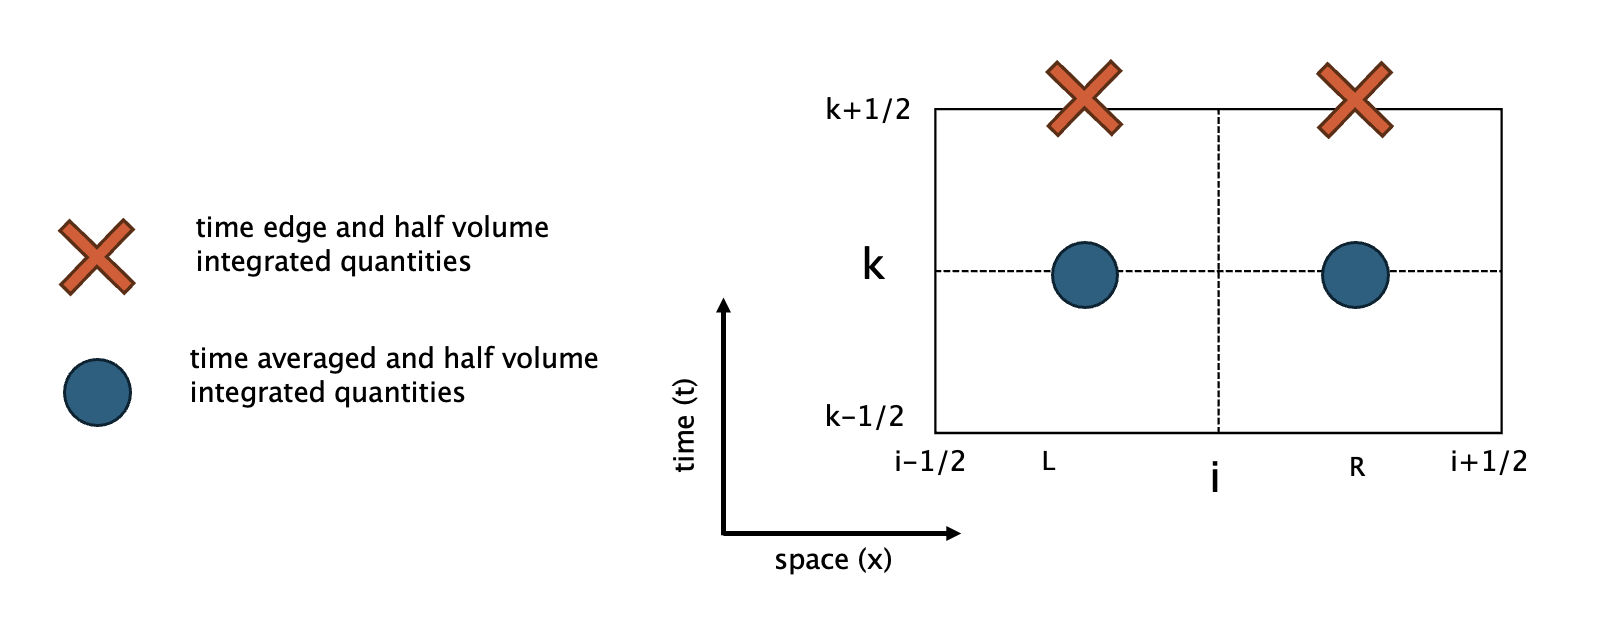
\includegraphics[width=\textwidth]{figures/stencil.png}
    \caption{The discretization stencil}
    \label{fig:stencil}
\end{figure}

%Figure \ref{fig:stencil} shows the stencil location for angular flux and source terms. 

In the traditional source iteration, the scattering source is presumed known from a previous iteration, which leads to the following set of equations to be solved in transport ``sweeps''.
This means that new estimates of both the end of time-step value of angular flux and time-averaged angular flux are computed together in each cell. 
So a $4\times4$ sized system (from stencil values) of equations must be solved to go from cell to cell in each angle.
This process is annoyingly serial over space, but embarrassingly parallel over angles.
The whole system sparse matrix is block (in each ordinate) lower triangular (over all cells).
Source iterations couple angles together in the iterative method by use of the scalar flux term.

In OCI, the scattering source is subtracted to the left-hand side, and the information that comes from cells other than cell $j$ is assumed to be known from a previous iteration.
This means that all $4NG$ angular fluxes ($N$ angles, $G$ groups, and stencil values $L$, $R$, $k$, $k+1/2$) are computed simultaneously in cell $j$.
For SCB in slab geometry, this means there is a local $4NG \times 4NG$ matrix to be solved in each cell.


\subsection{Fourier Analysis}

To ensure that our combination of higher-order discretization schemes is still unconditionally stable, we performed a Fourier analysis to find the slowest-converging mode of the method.
Assuming no scattering, no sources, homogeneous, mono-energetic problem, and make physical assumptions (only positive values of $\Delta x$, $\Delta t$, $\Sigma$, and $v$) we derived SCB-MB's eigen-function and numerically solve it. 
% \begin{subequations}
% \begin{align}
%     \psi_{k+1/2,j,L} &= \theta^{k+1}a e^{i\omega j}
%     &
%     \psi_{k+1/2,j,R} &= \theta^{k+1}b e^{i\omega j}
% \end{align}
% \begin{align}
%     \psi_{k,j,L} &= \theta^{k}c e^{i\omega j}
%     &
%     \psi_{k,j,R} &= \theta^{k}d e^{i\omega j}
% \end{align}
% \begin{align}
%     \psi_{k-1/2,j,L} &= \theta^{k}a e^{i\omega j}
%     &
%     \psi_{k-1/2,j,R} &= \theta^{k}b e^{i\omega j}
% \end{align}
% \end{subequations}
% where $k$ is the mode number, $i$ is the imaginary number, $\omega$ is the frequency of the mode, $\theta$ is the , and $j$ is the specific cell.
% Substituting our ansätze into Eqs.~\eqref{eq:scb-mb-a}, \eqref{eq:scb-mb-b}, \eqref{eq:scb-mb-c}, and \eqref{eq:scb-mb-d}, respectively, we
% When this system is solved for its eigenvalues ($\Lambda$) numerically it shows that a MB-SCB scheme is unconditionally stable over $\mu \in [-1, 1]$.  

\subsection{Verification using method of manufactured solution}

Finding benchmark problems that simulate transient, energy dependent, single dimension solutions to the neutron transport equation is difficult \cite{roy_review_2005}.
I used the Method of Manufactured solutions to derive my own benchmark \cite{nse_mms_warsaw}.
It is wildly accepted in the flied  and has previously been used to verify other deterministic neutron transport codes including the production code solver MOOSE \citep{wang_application_2018,moosemms}.

The method of manufactured solutions follow a backward solving technique where a solution is made-up---expressing any desired behavior (e.g. smoothness, differentiability, positivity, etc.)---then inserted into the governing equation and solved for the source term.
The manufactured source source is supplied to the solver to verify that it converges to the correct solution at the expected rate. 
To implement MMS I start with a manufactured continuous functional representation of the angular flux in angle, energy, space and time.
%\begin{subequations}
%    \label{eq:manufactured_sol}  
%    \begin{align}
%        \psi_1(x,t,\mu) = (1-\mu^2)\sin(\pi x)e^{-t} \label{eq:af_mms_cont1}\\
%        \psi_2(x,t,\mu) = (1-\mu^2)(-x^4 + x + 1)e^{-t/2} \label{eq:af_mms_cont2}
%    \end{align}
%\end{subequations} 
These equations can now be inserted into the NTE (eq \ref{eq:sn_nte}) and solved for a continuous functional representation of the source $Q$.
From there the source equations are placed on the stencil by averaging (via numerical integration) in space and time where necessary (see figure \ref{fig:stencil}).
This discretized set of sources is then supplied to the solver and the converged angular flux it provides is then compared to the original manufactured source (again placed on the stencil).
%The range we will be solving these equations is $x \in [0,1]$, $t \in [0,5]$ and $\mu \in [-1,1]$.
%Now we take \ref{eq:af_mms_cont1} and \ref{eq:af_mms_cont2} and insert them into the $S_N$ slab wall neutron transport equation defined in Eqn. \ref{eq:sn_nte} 
%\begin{subequations}
%        \begin{multline}
%            \frac{1}{v_1} \frac{\partial \psi_1(x,t,\mu)}{\partial t} + \mu \frac{\partial \psi_1 (x,t,\mu)}{\partial x} + \Sigma_1\psi_1(x,t,\mu)\\ 
%            =\frac{1}{2} \left(  \Sigma_{s,1} \int^1_{-1}\psi_1(x,t,\mu) \partial \mu + \Sigma_{s,2\rightarrow 1} \int^1_{-1}\psi_2(x,t,\mu) \partial \mu + Q_1\right) 
%        \end{multline}
%        and
%        \begin{multline}
%            \frac{1}{v_2} \frac{\partial \psi_2(x,t,\mu)}{\partial t} + \mu \frac{\partial \psi_2 (x,t,\mu)}{\partial x} + \Sigma_2\psi_2(x,t,\mu)\\ 
%            =\frac{1}{2} \left(  \Sigma_{s,2} \int^1_{-1}\psi_2(x,t,\mu) \partial \mu + \Sigma_{s,1\rightarrow 2} \int^1_{-1}\psi_1(x,t,\mu) \partial \mu + Q_2\right) 
%        \end{multline}
%\end{subequations}
%which yields continuous functional representations for solutions a source term,
%\begin{subequations}
%        \begin{equation}
%            Q_1(x,t,\mu) = \frac{2}{v_1} + 2\mu + 2\Sigma_1(\mu + t + x) - \Sigma_{S,1}(2t + 2x) - 2\Sigma_{S,2\rightarrow1}tx^2 
%        \end{equation}
%        and
%        \begin{equation}
%            Q_2(x,t,\mu) = \frac{2x^2}{v_2} + 4\mu tx + 2\Sigma_2(\mu + tx^2) + \Sigma_{S,1\rightarrow2}(2t + 2x) - 2\sigma_{S,2}tx^2
%        \end{equation}
%\end{subequations}
%Note that these equations are fully defined by independent variables and material data.


\subsection{Implementation in code}

I use the ROCm compute library to solve the system of equations.
Modern GPU vendor supplied LAPACK libraries often include a \texttt{strided\_batched} class of solvers.
These will operate on a group of like-sized systems in unison and are optimized by the vendors of the hardware themselves.
For example, LU decomposition with pivoting (the most generic direct solver for a system of linear equations) is implemented using RocSolvers \texttt{strided\_batched\_dgsev}.
Direct solvers where used in this work because all systems where smallish (with orders ranging between 4 and 1000).
%Spare direct solvers could be utilized in the future to decrease memory footprint of OCI schemes specifically.
This makes the use of a strided batched implementation of LU decomposition with pivoting ideal.
Furthermore in this work once that system is solved once the return of the A matrix is automatically L+U+D.
In subsequent iterations this system can be back solved very quickly.
For both schemes the entire convergence loop was executed on the GPU.

\subsection{Exploration of acceleration scheme}
\label{ssec:method_acc}

This section discusses ongoing work: the derivation of an acceleration scheme for OCI in the thin limit.
When working with the iterative schemes it becomes useful to define systems in operator notation.
The NTE can be written generally as
\begin{equation}
    H\psi = q
\end{equation}
where $H$ is some invertible operator, $\psi$ is the unknown function for angular flux and $q$ is some source.
To solve this equation we split H into components that makes sense given the NTE, then let something lag and something lead (assuming a fixed point iteration).
How that operator is split is what differentiates OCI from SI.
For example if we choose $H = L-S$ where $L$ is the left hand side of the transport equation and $S$ is the scattering source and finally let the fluxes on the source lag we get
\begin{equation}
    L\psi^{l+1} = S\psi^l + q
\end{equation}
which is a source iteration.
For now we will start with OCI's operator notation from Rosa, Warsaw, and Perks (2013) \cite{rosa_cellwise_2013} which they call cellwise-bJ
\begin{equation}
    \label{eq:operator_nte}
    (L-S)\psi = q
\end{equation}
where $L$ = streaming thru space and time and total integration operator, %\\ ($\mu_m\frac{\partial\psi}{\partial x} + \frac{1}{v}\frac{\partial\psi}{\partial t} + \Sigma \psi$)
$S$ is the scattering operator (discrete-to-moment operator) which couples all the simultaneous PDEs together, %\\($\Sigma_s \int^1_{-1}\psi\partial\mu = \Sigma_s \sum_{n=0}^{M}w_n\psi_n = \Sigma_s\phi$)
$\psi$ angular flux (dependent variable of interest), and
$q$ is the fixed material source.
OCI works by lagging the incident cell wall fluxes of the cell.
Those flux come from the upstream closure that transport solvers use.
Thus it is convenient to define,
\begin{equation}
    L = L_c + L_b
\end{equation}
where $L_c$ are the angular fluxes within a mesh cell and $L_b$ are the angular fluxes incident to the mesh cell's surface.
    %\\($\mu_m\psi_b\frac{dA}{dx} + \frac{1}{v}\psi_b\frac{dA}{dx}$)
Note that what $L_b$ actually consists of depends on the space discretization.
After this operator splitting equation \ref{eq:operator_nte} now becomes
\begin{equation}
    \psi[I+(L_c-S)^{-1}L_b] = (L_c-S)^{-1}q
\end{equation}
where I is the identity matrix.
When we prescribe what lags in OCI (incident fluxes on the surface of the cell) this becomes
\begin{equation}
    \label{eq:itter}
    \psi^{(l+1)} = (L_c-S)^{-1}(-L_b\psi^l+q)
\end{equation}

When looking for an acceleration scheme examining the structure of $L_b$ becomes important.
In my research I use the TDMB+SCB discretization for time dependent single dimension multi-group Sn problems (equation \ref{eq:tdmb+scb}).
If the angular fluxes from the boundary of the cell are identified (denoted by $j\pm1/2$) we can identify $L_b$'s structure generally.
It should be something like $\pm\mu_m$ filled along four diagonals with every 4th space filled.
This is also similar to how the SI equations look if formed as a lower triangular system.
In higher dimensions I expect the structure to remain mostly the same for rectilinear grids but might get more complex for unstructured meshes where surface areas may become an issue.
For now we generally know the structure of $L_b$

Next lets think about the within cell operator $L_c$.
We know $L_c$ contains the differential and absorption terms from the NTE.
We know that OCI converges in the thin limit due to a-synchronicity \cite{rosa_cellwise_2013, hoagland_hybrid_2021}, measured in mean-free paths (MFP)s.
So I know a small MFP leads to a large condition number of our iteration matrix, and thus slow convergence.
To isolate this term we start with
\begin{equation}
    L_c = K_d + K_a
\end{equation}
where $K_d$ is the differential operators and absorption term:
\begin{equation}
    K_a = \frac{\Delta x \Sigma}{2}  I
\end{equation}
$K_a$'s structure is pretty easy to identify from the equations \ref{eq:tdmb+scb}.
I could pull out a solitary $\Sigma$ but in this form I can identify that
\begin{equation}
    K_a = \frac{\text{MFP}}{2}  I
\end{equation}
Pushing forward I break up our equations into a standard synthetic approach.
I start with equation \ref{eq:itter} but recast it with some of the expansions I just identified,
\begin{equation}
    \psi^{l+1}(K_d + \delta I - S) = (-L_b\psi^l + q)
\end{equation}
where $\delta=$ MFP$/2$. Now we can write the associated equation for the iteration error as,
\begin{equation}
    (K_d + \delta I-S) f^{l+1} = -L_b f^l
\end{equation}
where $f^{l+1} = \psi^{\text{converged}}-\psi^{l+1/2}$ and $f^{l} = \psi^{\text{converged}}-\psi^{l}$.
Note that this equation is exact in it's current forum.
Now we use $-L_bf^{l-1}$ as our special one and subtract from both sides
\begin{equation}
    (K_d + \delta I - S + L_b)f^{l+1} = L_b(f^{l+1}-f^l)
\end{equation}
Notably here if we re-add everything back together we should still have equation \ref{eq:itter}.
Now we can formally set up our synthetic-two-step starting with equation \ref{eq:itter} rewritten for half steps
\begin{subequations}
    \begin{equation}
        \label{eq:acc1}
        \psi^{(l+1/2)} = (L_c-S)^{-1}(-L_b\psi^l+q)
    \end{equation}  
    the associated equation for mid step error
    \begin{equation}  
        \label{eq:acc2}
        f^{l+1/2} = -M L_b(\psi^{l+1/2}-\psi^l)
    \end{equation}  
    and the definition of the errors
    \begin{equation}  
        \label{eq:acc3}
        \psi^{l+1} = \psi^{l+1/2} + f^{l+1/2}
    \end{equation}
\end{subequations}
where,
\begin{equation}
    M \approx (K_d + \delta I + L_b - S)^{-1}
\end{equation}
and is easier to obtain then the actual inverse.
Note that eq 3 from ref \cite{tsa2009rosa} is the recombined version of eq \ref{eq:acc2}.
From here estimations can be made about what a good approximate of $M$ will be in the conditions where \ref{eq:acc1} degrades.
%If we actually inverted $H$ this would just be another transport step.
%Note that we can relate this idea of synthetic acceleration to preconditioning by noting
%\begin{equation}
%    P \equiv I + M(I-H)
%\end{equation}
%From here I take some stabs at identifying what reasonable values for $M$ could be.
%When we ask our selves "what should M be" we could just as easily pose the more pessimistic analog: "why or, where rather, does H suck to invert".
%This is where our knowledge about the thin limit comes in.
%We know H is painful to invert when $\delta I$ is small as that is a problem in the thin limit where cell wise communication becomes dominant.
%When $\delta I$ is small a good conservative approximation for M may become
%\begin{equation}
%    H^{-1} \approx M = (K_d + L_b - S)^{-1}
%\end{equation}
%but we just converged our within-cell scattering, time rate of change, and steaming operators from the transport step so lets assume we have a good estimate of that.
%We can also assume that the boundary information coming into every cell will blah likewise lets scoot that and all we are left with is the differential operators (from a discretization scheme)
%\begin{equation}
%    H^{-1} \approx M = (K_d)^{-1}
%\end{equation}
%which makes the full mid step solution
%\begin{equation}
%    \label{eq:m}
%    -K_d^{-1}*L_b
%\end{equation}
%This leads to the suggestion at the possible algorithm
%\begin{enumerate}
%    \item transport step as described in eq. \ref{eq:acc1}
%    \item mid step corrector (eq. \ref{eq:acc2}) with . This will look like a transport in every angle
%    \item colsure from eq
%\end{enumerate}
%But Joanna, your probably asking yourself. 
%This just using a cheap sweep between every OCI transport iteration
%I say in 1D
%in higher dimensions this will look like a \textit{a ray trace} something GPUs are literally built for.

%From here more work is need to be down to conduct Fourier analysis in both with and with out the discretization scheme

%What ever scheme is used it can be supplemented by GMRES

\section{Monte Carlo transport methods}
As in the previous section the methods employed are described in attached publications in the appendix.
They are beefily summarized here but far more information is contained there for the edification of the reader.

%   
\subsection{Python based portability for rapid methods development}

A software engineering scheme was developed and deployed in Monte Carlo/Dynamic Code \cite{morgan_monte_2024} using the Numba compiler for Python \cite{lam_numba_2015}, mpi4py \cite{mpi4py_2021}, and an a-synchronous GPU event scheduler called Harmonize \cite{brax2023} (\textit{see appendix \ref{app:cise}}).
MC/DC can run the same set of physics functions written by subject-area experts in the Python interpreter or compiled to x86-64, ARM64, Power9 CPUs and AMD and Nvidia GPUs.
All compilation targets also support the use of MPI to distribute work to multiple nodes of an HPC.
It is a demonstration of portability using a high-level language coupled to a portability framework to enable rapid methods development.

\subsection{Delta tracking in MCATK and MC/DC}

In MCATK a hybrid delta-surface tracking scheme was developed and deployed (\textit{see appendix \ref{app:hybridmcatk}}).
I initially implemented this scheme upto the work presented, but it has been extended by others and is shipped in current production versions of MCATK.
The point of the delta-surface tracking scheme in MCATK was entirely to avoid extra macroscopic cross section lookups.
It still conducted surface tracking on mesh.
After implementation the hybrid delta-tracking scheme was tested in both k-eigenvalue and fixed source transient simulations using the,
\begin{itemize}
    \item HEU-MET-FAST-086 benchmark of Godiva IV \cite{godivaiv2021}; and
    \item Measurement of Uranium Subcritical and Critical IER 488 (MUSiC) experiment \cite{music2021}.
\end{itemize}
Runtime and errors were then compared to draw conclusions.
This work was published in a conference publication \cite{morgan2023oci} (\textit{see appendix \ref{app:cise}}).

In MC/DC I propose a slight alteration to the hybrid-scheme developed and deployed in my previous work in MCATK.
Current versions of MC/DC do not stop particles at mesh crossings and uses a track-length estimator to tally impacts to multiple cells at once.
Using this algorithm already in MC/DC, delta tracking could be used in conjunction with the track length estimator as in the previous work in MCATK.
However the proposed algorithm in MC/DC will more closely resemble the vanilla delta tracking algorithm and not stop particles at now cell and surface crossings.
Other quantities of interest will be tallied with collision estimator as the specific material data is required for values like fission reaction rate.
This will require additional computational burden but the hope is that the new tally functionality in MC/DC is sufficiently optimized to still allow this scheme to be more performant.

To evaluate the delta tracking scheme as compared to surface tracking I will use figure of merit (FOM) values.
FOMs are constructed to observe impact of a variance reduction technique on both variance (as computed by the Monte Carlo scheme) and on runtime (as many variance reduction schemes incur additional computation burden).
The most common figure of merit and the one I will employ is simply
\begin{equation}
    FOM = \frac{1}{\sigma^2 t_{wc}}
\end{equation}
where $\sigma^2$ is the variance as already computed by MC solvers and $t_{wc}$ is the total wall-clock-runtime.
Using this metric (higher is better) variance reduction shames can be compared to each other and the analog solver.
I propose using this metric to evaluate the impact of the hybrid-delta tracking scheme I plan to implement in MC/DC in a problem of interest.
Potential problems of interest include:
\begin{enumerate}
    \item Dragon burst problem \cite{kimpland2021dragon};
    \item C5G7 Small modular reactor \cite{jia_hou_oecdnea_2017}; and
    \item Kobyashi void dog-leg void problem (multigroup and contentious energy simulations) \cite{Kobayashi2001}.
\end{enumerate}